\chapter{La mole et la masse molaire}\label{ch:g10:the-mole}

En fin de journée, une banque ne compte pas ses pièces une à une~: elle
les pèse. Si une pièce a une masse de \qty{7.5}{g}, un sac de pièces de
\qty{7.5}{kg} en contient mille, et c'est la balance qui a compté. Les
chimistes ont le même problème avec les \omterm{def:g7:atoms-and-molecules:atom}{atomes}, en bien pire~: une
cuillerée d'eau contient plus de \omterm{def:g7:atoms-and-molecules:molecule}{molécules} qu'il n'y a de grains de
sable sur toutes les plages d'une côte. Ils le résolvent de la même
façon, en pesant, et le sac qu'ils utilisent contient
\num{602214076000000000000000} entités. Ce chapitre définit ce sac, la
\omterm{def:g10:the-mole:amount}{mole}, et montre comment passer d'une masse lue sur une balance à un
nombre d'\omterm{def:g7:atoms-and-molecules:atom}{atomes} ou de \omterm{def:g7:atoms-and-molecules:molecule}{molécules}.

\begin{recall}
La masse d'un \omterm{def:g7:atoms-and-molecules:atom}{atome} est concentrée dans son \omterm{def:g9:inside-the-atom:nucleus}{noyau}~; un \omterm{def:g9:inside-the-atom:proton}{proton} et un
\omterm{def:g9:inside-the-atom:proton}{neutron} ont chacun une masse d'environ \qty{1.67e-27}{kg}, si bien qu'un
\omterm{def:g7:atoms-and-molecules:atom}{atome} de \omterm{def:g9:inside-the-atom:atomic-number}{nombre de masse} $A$ a une masse d'environ
$A \times \qty{1.67e-27}{kg}$. Les très grands et les très petits
nombres s'écrivent en écriture scientifique
(\cref{ch:g9:inside-the-atom}). Une \omterm{def:g7:atoms-and-molecules:formula}{formule chimique} donne le nombre
d'\omterm{def:g7:atoms-and-molecules:atom}{atomes} de chaque élément dans une \omterm{def:g7:atoms-and-molecules:molecule}{molécule}
(\cref{ch:g7:atoms-and-molecules}).
\end{recall}

\begin{omfigure}
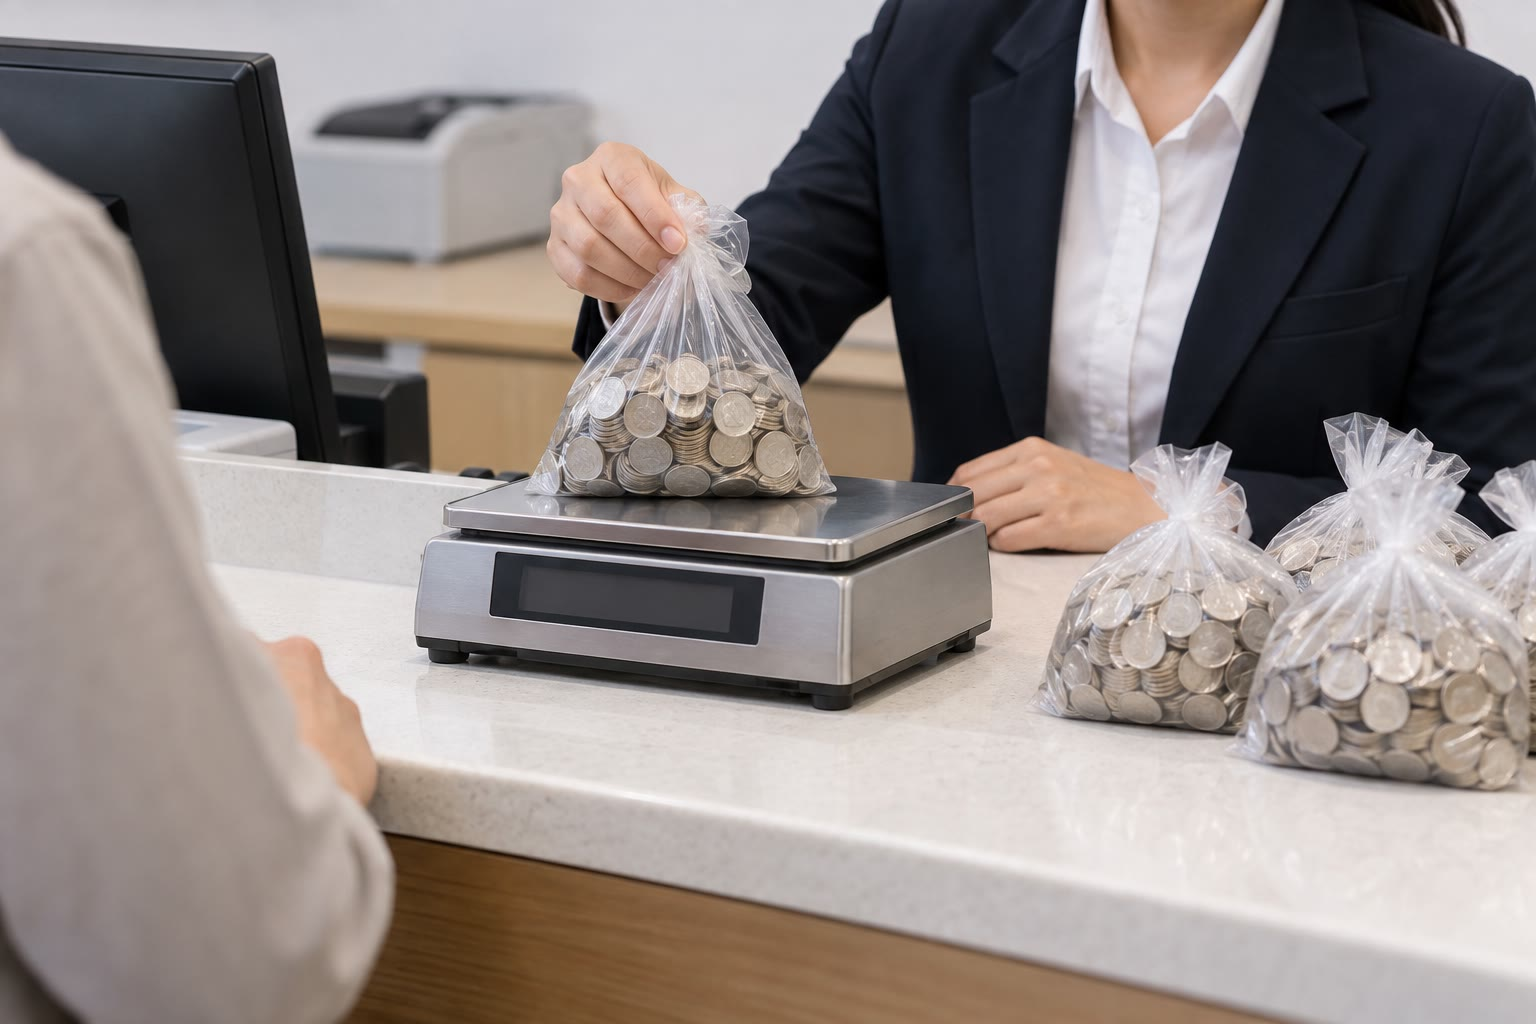
\includegraphics[width=0.55\linewidth]{images/book1/ai/g10-bank-coins.jpg}

{\small Une banque compte les pièces en les pesant. Les chimistes
comptent les \omterm{def:g7:atoms-and-molecules:atom}{atomes} de la même façon.}
\end{omfigure}

\section{Compter en pesant}

\begin{example}[Un sac de pièces]\label{ex:g10:the-mole:coins}
Une pièce a une masse de \qty{7.5}{g}. Un sac de ces pièces a une masse
de \qty{1.80}{kg}, soit \qty{1800}{g}, la masse du sac lui-même étant
mise à part. Il contient
\[
  \frac{\qty{1800}{g}}{\qty{7.5}{g}} = 240 \text{ pièces.}
\]
Pour compter, la banque divise la masse totale par la masse d'une pièce.
\end{example}

\begin{example}[Une cuillerée d'eau]\label{ex:g10:the-mole:spoon}
Une \omterm{def:g7:atoms-and-molecules:molecule}{molécule} d'eau, \ce{H2O}, compte $2 + 16 = 18$ \omterm{def:g9:inside-the-atom:proton}{nucléons} (les \omterm{def:g7:atoms-and-molecules:atom}{atomes}
d'oxygène~16 et d'hydrogène~1 forment presque toute l'eau naturelle)~;
sa masse est donc d'environ
$18 \times \qty{1.67e-27}{kg} = \qty{3.0e-26}{kg}$, soit
\qty{3.0e-23}{g}. Une cuillerée de \qty{5.0}{g} d'eau contient donc
\[
  \frac{\qty{5.0}{g}}{\qty{3.0e-23}{g}} \approx \num{1.7e23}
  \text{ molécules.}
\]
La division se fait comme pour les pièces, mais le résultat est un
nombre que personne ne peut se représenter. Les chimistes ont besoin
d'un paquet d'\omterm{def:g7:atoms-and-molecules:atom}{atomes} adapté aux échantillons du laboratoire.
\end{example}

\begin{definition}[Quantité de matière et mole]\label{def:g10:the-mole:amount}
% ledger: const:NA
La \emph{quantité de matière}\index{quantite de matiere@quantité de matière} $n$ d'un
échantillon compte les entités qu'il contient (\omterm{def:g7:atoms-and-molecules:atom}{atomes}, \omterm{def:g7:atoms-and-molecules:molecule}{molécules} ou
\omterm{def:g9:ions:ion}{ions}, à préciser chaque fois). Son unité est la \emph{mole}\index{mole},
de symbole \si{mol}~: une mole contient exactement
\num{6.02214076e23} entités.
\end{definition}

\begin{remark}[Une douzaine, une rame, une mole]\label{rem:g10:the-mole:dozen}
La \omterm{def:g10:the-mole:amount}{mole} est une unité de comptage, comme une douzaine d'œufs (12) ou
une rame de papier (500 feuilles), en beaucoup plus grand. «~Deux \omterm{def:g10:the-mole:amount}{moles}
de \omterm{def:g7:atoms-and-molecules:molecule}{molécules} d'eau~» signifie $2 \times \num{6.02214076e23} = \num{1.20e24}$
\omterm{def:g7:atoms-and-molecules:molecule}{molécules}, de même que «~deux douzaines d'œufs~» signifie 24 œufs. Il
faut toujours préciser quelles entités on compte~: une \omterm{def:g10:the-mole:amount}{mole} de
\emph{\omterm{def:g7:atoms-and-molecules:molecule}{molécules}} de dioxygène \ce{O2} contient deux \omterm{def:g10:the-mole:amount}{moles}
d'\emph{\omterm{def:g7:atoms-and-molecules:atom}{atomes}} d'oxygène.
\end{remark}

\begin{history}[L'hypothèse d'Avogadro, 1811]
En 1811, le physicien Amedeo Avogadro proposa que des volumes égaux de
gaz différents, à la même température et à la même pression, contiennent
le même nombre de particules. Il comprit aussi qu'un gaz comme le
dioxygène est fait de \omterm{def:g7:atoms-and-molecules:molecule}{molécules} de deux \omterm{def:g7:atoms-and-molecules:atom}{atomes}. Son idée fut négligée
pendant près de cinquante ans, jusqu'à ce que Stanislao Cannizzaro
l'utilise en 1860 pour obtenir un ensemble cohérent de masses atomiques.
La constante qui compte les entités d'une \omterm{def:g10:the-mole:amount}{mole} reçut plus tard le nom
d'Avogadro~; il n'en connut jamais la valeur.
\end{history}

\begin{omfigure}
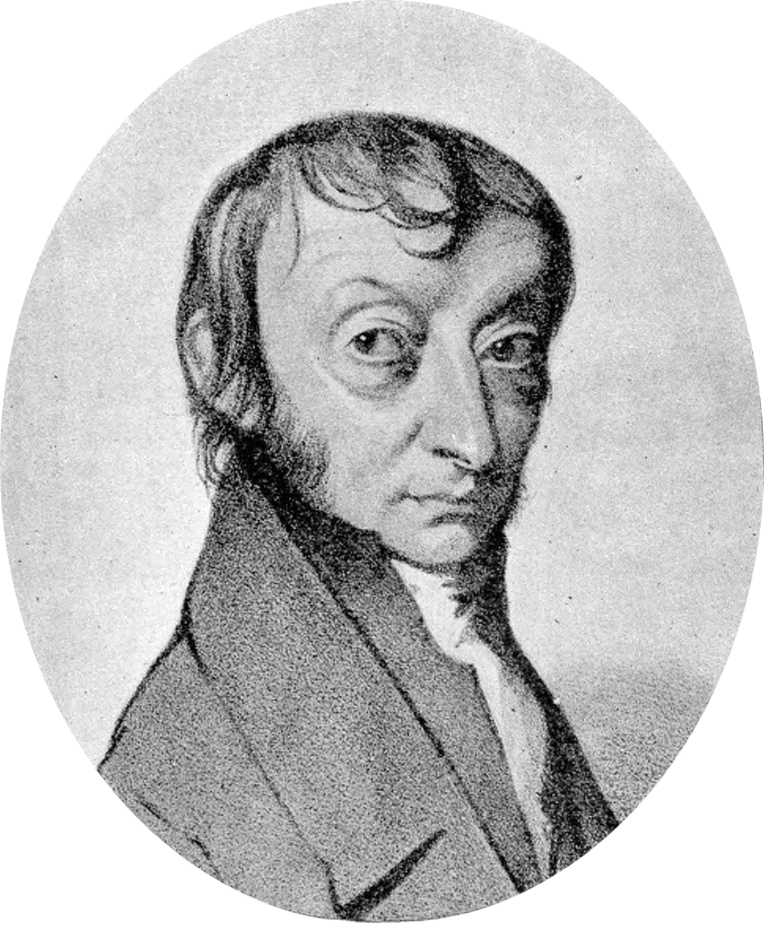
\includegraphics[width=0.26\linewidth]{images/book1/avogadro.jpg}

{\small Amedeo Avogadro (1776--1856).}
\end{omfigure}

\section{La constante d'Avogadro}

\begin{definition}[Constante d'Avogadro]\label{def:g10:the-mole:avogadro}
% ledger: const:NA
La \emph{constante d'Avogadro}\index{constante d'Avogadro} $N_A$ est le
nombre d'entités par \omterm{def:g10:the-mole:amount}{mole}~:
\[
  N_A = \qty{6.02214076e23}{mol^{-1}} .
\]
Sa valeur est exacte, fixée par définition. Dans les calculs, on
l'arrondit à \qty{6.02e23}{mol^{-1}}.
\end{definition}

\begin{proposition}[Nombre d'entités et quantité de matière]\label{prop:g10:the-mole:number}
Un échantillon contenant $N$ entités contient la \omterm{def:g10:the-mole:amount}{quantité de matière}
\[
  n = \frac{N}{N_A}, \qquad\text{soit}\qquad N = n \times N_A .
\]
\end{proposition}

\begin{proof}
Chaque \omterm{def:g10:the-mole:amount}{mole} contient $N_A$ entités, donc $n$ \omterm{def:g10:the-mole:amount}{moles} contiennent
$n \times N_A$ entités~; en divisant par $N_A$, on obtient $n$.
\end{proof}

\begin{example}[Molécules et moles]\label{ex:g10:the-mole:convert}
Un échantillon contient \num{1.5e24} \omterm{def:g7:atoms-and-molecules:molecule}{molécules} de dioxyde de carbone. Sa
quantité de dioxyde de carbone est
$n = \num{1.5e24} / \qty{6.02e23}{mol^{-1}} = \qty{2.5}{mol}$.
Inversement, \qty{0.20}{mol} de fer contiennent
$N = \qty{0.20}{mol} \times \qty{6.02e23}{mol^{-1}} = \num{1.2e23}$
\omterm{def:g7:atoms-and-molecules:atom}{atomes} de fer.
\end{example}

\begin{remark}[D'où vient ce nombre]\label{rem:g10:the-mole:origin}
Pendant plus de cinquante ans, la \omterm{def:g10:the-mole:amount}{mole} a été définie comme le nombre
d'\omterm{def:g7:atoms-and-molecules:atom}{atomes} contenus dans exactement \qty{12}{g} de carbone~12, et $N_A$
devait être mesurée. Depuis 2019, c'est le nombre lui-même qui est fixé,
ce qui fait de la \omterm{def:g10:the-mole:amount}{mole} un pur comptage. L'ancienne et la nouvelle
définition concordent à mieux qu'une partie sur cent millions~: douze
grammes de carbone~12 contiennent donc toujours une \omterm{def:g10:the-mole:amount}{mole} d'\omterm{def:g7:atoms-and-molecules:atom}{atomes}, comme
le vérifie la section suivante.
\end{remark}

\section{La masse molaire}

\begin{definition}[Masse molaire]\label{def:g10:the-mole:molar-mass}
La \emph{masse molaire}\index{masse molaire} $M$ d'une \omterm{def:g6:pure-substances-and-mixtures:species}{espèce chimique}
est la masse d'une \omterm{def:g10:the-mole:amount}{mole} de ses entités, en grammes par \omterm{def:g10:the-mole:amount}{mole}
(\si{g/mol}). La masse molaire d'un élément, prise sur son \omterm{def:g6:pure-substances-and-mixtures:mixture}{mélange}
naturel d'\omterm{def:g9:inside-the-atom:isotope}{isotopes}, est sa
\emph{masse molaire atomique}\index{masse molaire atomique}~; elle figure
dans le \omterm{def:g9:periodic-table-first-look:periodic-table}{tableau périodique}.
\end{definition}

\begin{example}[Une mole d'atomes de carbone]\label{ex:g10:the-mole:carbon}
% ledger: const:NA, const:u
Un \omterm{def:g7:atoms-and-molecules:atom}{atome} de carbone~12 a une masse d'environ
$12 \times \qty{1.67e-27}{kg} = \qty{2.00e-26}{kg}$. Une \omterm{def:g10:the-mole:amount}{mole} de ces
\omterm{def:g7:atoms-and-molecules:atom}{atomes} a une masse de
\[
  \qty{2.00e-26}{kg} \times \num{6.02e23} = \qty{1.20e-2}{kg}
  = \qty{12.0}{g}.
\]
La \omterm{def:g10:the-mole:amount}{mole} a été choisie pour que la \omterm{def:g10:the-mole:molar-mass}{masse molaire} d'un \omterm{def:g7:atoms-and-molecules:atom}{atome}, en grammes
par \omterm{def:g10:the-mole:amount}{mole}, soit proche de son \omterm{def:g9:inside-the-atom:atomic-number}{nombre de masse}~: environ \qty{1}{g/mol}
pour l'hydrogène, \qty{12}{g/mol} pour le carbone, \qty{16}{g/mol} pour
l'oxygène.
\end{example}

\begin{omfigure}
% ledger: aw:H, aw:C, aw:N, aw:O, aw:Na, aw:Mg, aw:Al, aw:Si, aw:S, aw:Cl, aw:K, aw:Ca, aw:Fe, aw:Cu, aw:Zn, aw:Au (rounded to 0.1)
\begin{tabular}{lcr@{\qquad}lcr}
\hline
élément & symbole & $M$ (\si{g/mol}) & élément & symbole & $M$ (\si{g/mol}) \\
\hline
hydrogène & \ce{H}  & 1.0  & silicium  & \ce{Si} & 28.1 \\
carbone   & \ce{C}  & 12.0 & soufre    & \ce{S}  & 32.1 \\
azote     & \ce{N}  & 14.0 & chlore    & \ce{Cl} & 35.5 \\
oxygène   & \ce{O}  & 16.0 & potassium & \ce{K}  & 39.1 \\
sodium    & \ce{Na} & 23.0 & calcium   & \ce{Ca} & 40.1 \\
magnésium & \ce{Mg} & 24.3 & fer       & \ce{Fe} & 55.8 \\
aluminium & \ce{Al} & 27.0 & cuivre    & \ce{Cu} & 63.5 \\
          &         &      & or        & \ce{Au} & 197.0 \\
\hline
\end{tabular}\par\medskip

{\small \omterm{def:g10:the-mole:molar-mass}{Masses molaires atomiques} d'éléments courants, arrondies à
\qty{0.1}{g/mol}. Ce sont les valeurs utilisées dans ce livre.}
\end{omfigure}

\begin{remark}[Pourquoi le chlore vaut 35.5]\label{rem:g10:the-mole:chlorine}
% ledger: iso:Cl35, iso:Cl37
Le chlore naturel est un \omterm{def:g6:pure-substances-and-mixtures:mixture}{mélange} de deux \omterm{def:g9:inside-the-atom:isotope}{isotopes}~: environ les trois
quarts de ses \omterm{def:g7:atoms-and-molecules:atom}{atomes} sont du chlore~35, un quart du chlore~37
(\cref{ch:g9:inside-the-atom}). Sa \omterm{def:g10:the-mole:molar-mass}{masse molaire atomique} est la
moyenne pondérée par ces proportions, qui se situe entre 35 et 37~:
\qty{35.5}{g/mol}. C'est pourquoi certaines \omterm{def:g10:the-mole:molar-mass}{masses molaires atomiques}
sont loin d'être des nombres entiers.
\end{remark}

\begin{proposition}[Masse molaire d'une molécule]\label{prop:g10:the-mole:sum}
La \omterm{def:g10:the-mole:molar-mass}{masse molaire} d'une \omterm{def:g7:atoms-and-molecules:molecule}{molécule} est la somme des \omterm{def:g10:the-mole:molar-mass}{masses molaires
atomiques} de tous ses \omterm{def:g7:atoms-and-molecules:atom}{atomes}, chacun compté autant de fois qu'il apparaît
dans la formule. La même règle donne la \omterm{def:g10:the-mole:molar-mass}{masse molaire} d'un solide ionique
à partir de son unité de formule.
\end{proposition}

\begin{proof}
Une \omterm{def:g10:the-mole:amount}{mole} de \omterm{def:g7:atoms-and-molecules:molecule}{molécules} \ce{A_xB_y} contient $x$ \omterm{def:g10:the-mole:amount}{moles} d'\omterm{def:g7:atoms-and-molecules:atom}{atomes} \ce{A} et
$y$ \omterm{def:g10:the-mole:amount}{moles} d'\omterm{def:g7:atoms-and-molecules:atom}{atomes} \ce{B}, et rien d'autre~; sa masse est la somme de
leurs masses, $x\,M(\ce{A}) + y\,M(\ce{B})$.
\end{proof}

\begin{example}[Trois masses molaires]\label{ex:g10:the-mole:three}
% ledger: aw:H, aw:C, aw:O, aw:Na, aw:Cl
\begin{align*}
  M(\ce{H2O}) &= 2 \times 1.0 + 16.0 = \qty{18.0}{g/mol},\\
  M(\ce{NaCl}) &= 23.0 + 35.5 = \qty{58.5}{g/mol},\\
  M(\ce{C12H22O11}) &= 12 \times 12.0 + 22 \times 1.0 + 11 \times 16.0
     = \qty{342.0}{g/mol}.
\end{align*}
La dernière est celle du saccharose, le sucre de table.
\end{example}

\section{De la masse à la quantité de matière, et retour}

\begin{proposition}[Masse et quantité de matière]\label{prop:g10:the-mole:mass}
Un échantillon de masse $m$ d'une espèce de \omterm{def:g10:the-mole:molar-mass}{masse molaire} $M$ contient la
\omterm{def:g10:the-mole:amount}{quantité de matière}
\[
  n = \frac{m}{M}, \qquad\text{soit}\qquad m = n \times M .
\]
Avec $m$ en grammes et $M$ en grammes par \omterm{def:g10:the-mole:amount}{mole}, $n$ est en \omterm{def:g10:the-mole:amount}{moles}.
\end{proposition}

\begin{proof}
Chaque \omterm{def:g10:the-mole:amount}{mole} a une masse $M$, donc $n$ \omterm{def:g10:the-mole:amount}{moles} ont une masse $n \times M$~;
c'est le comptage des pièces de la banque, avec la \omterm{def:g10:the-mole:amount}{mole} pour pièce.
\end{proof}

\begin{method}[D'une masse à un nombre d'entités]\label{met:g10:the-mole:mass-to-number}
\begin{enumerate}
  \item Écrire la formule de l'espèce et calculer sa \omterm{def:g10:the-mole:molar-mass}{masse molaire} $M$ à
        l'aide du tableau.
  \item Convertir la masse en grammes si nécessaire, puis $n = m / M$.
  \item Si l'on cherche le nombre d'entités, $N = n \times N_A$.
  \item Vérifier l'ordre de grandeur~: quelques grammes d'une petite
        \omterm{def:g7:atoms-and-molecules:molecule}{molécule} représentent de l'ordre d'un dixième de \omterm{def:g10:the-mole:amount}{mole}, soit
        $10^{22}$ à $10^{23}$ entités.
\end{enumerate}
\end{method}

\begin{omfigure}
\begin{tikzpicture}[font=\small, box/.style={draw=omDef, very thick,
    fill=omDef!8, rounded corners=3pt, minimum width=2.9cm,
    minimum height=1.1cm, align=center}]
  \node[box] (m) at (0,0) {masse $m$\\[1pt] (\si{g})};
  \node[box] (n) at (5,0) {quantité $n$\\[1pt] (\si{mol})};
  \node[box] (N) at (10,0) {nombre $N$\\[1pt] d'entités};
  \draw[-{Stealth[length=7pt]}, thick, omProp] ([yshift=4pt]m.east)
    -- node[above] {$\div M$} ([yshift=4pt]n.west);
  \draw[-{Stealth[length=7pt]}, thick, omProp] ([yshift=-4pt]n.west)
    -- node[below] {$\times M$} ([yshift=-4pt]m.east);
  \draw[-{Stealth[length=7pt]}, thick, omProp] ([yshift=4pt]n.east)
    -- node[above] {$\times N_A$} ([yshift=4pt]N.west);
  \draw[-{Stealth[length=7pt]}, thick, omProp] ([yshift=-4pt]N.west)
    -- node[below] {$\div N_A$} ([yshift=-4pt]n.east);
\end{tikzpicture}

{\small La \omterm{def:g10:the-mole:amount}{quantité de matière} $n$ est au centre~: la balance donne $m$,
la \omterm{def:g10:the-mole:molar-mass}{masse molaire} conduit à $n$, et la \omterm{def:g10:the-mole:avogadro}{constante d'Avogadro} conduit
ensuite au nombre d'entités.}
\end{omfigure}


\begin{example}[Neuf grammes d'eau]\label{ex:g10:the-mole:nine}
% ledger: aw:H, aw:O, const:NA
Combien y a-t-il de \omterm{def:g7:atoms-and-molecules:molecule}{molécules} dans \qty{9.0}{g} d'eau~? $M(\ce{H2O}) =
\qty{18.0}{g/mol}$, donc
\[
  n = \frac{\qty{9.0}{g}}{\qty{18.0}{g/mol}} = \qty{0.50}{mol},
  \qquad
  N = \qty{0.50}{mol} \times \qty{6.02e23}{mol^{-1}}
    = \num{3.0e23} \text{ molécules.}
\]
\end{example}

\begin{example}[Une mole sur la paillasse]\label{ex:g10:the-mole:bench}
% ledger: rho:water, rho:NaCl, rho:sucrose, rho:Fe, aw:H, aw:O, aw:Na, aw:Cl, aw:C, aw:Fe
Une \omterm{def:g10:the-mole:amount}{mole} d'eau, c'est \qty{18.0}{g}, environ une cuillerée à soupe. Une
\omterm{def:g10:the-mole:amount}{mole} de sel, \qty{58.5}{g}, forme un petit tas~; une \omterm{def:g10:the-mole:amount}{mole} de sucre,
\qty{342.0}{g}, remplit une grande tasse~; une \omterm{def:g10:the-mole:amount}{mole} de fer,
\qty{55.8}{g}, est un cube d'un peu moins de \qty{2}{cm} de côté. Les
quatre contiennent le même nombre d'entités~: les \omterm{def:g7:atoms-and-molecules:molecule}{molécules} de sucre
sont simplement bien plus lourdes que celles d'eau, et les \omterm{def:g7:atoms-and-molecules:atom}{atomes} de
fer sont bien plus serrés.
\end{example}

\begin{omfigure}
\begin{tikzpicture}[font=\small, x=0.62cm, y=0.62cm]
  % cubes of true volume, drawn to one common scale: side = cube root of V
  % water 18.09 cm3 -> 2.625 cm; NaCl 26.96 cm3 -> 2.999 cm;
  % sucrose 216.4 cm3 -> 6.004 cm; Fe 7.09 cm3 -> 1.921 cm
  \newcommand{\cube}[4]{% x, side, fill, label
    \pgfmathsetmacro\d{0.35*#2}
    \fill[#3!35, draw=#3!80!black] (#1,0) rectangle ++(#2,#2);
    \fill[#3!20, draw=#3!80!black] (#1,#2) -- ++(\d,\d) -- ++(#2,0)
      -- ++(-\d,-\d) -- cycle;
    \fill[#3!50, draw=#3!80!black] (#1+#2,0) -- ++(\d,\d) -- ++(0,#2)
      -- ++(-\d,-\d) -- cycle;
    \node[below, align=center] at (#1+#2/2,-0.1) {#4};}
  \cube{0}{2.625}{cyan}{eau\\ \qty{18.0}{g}\\ \qty{18}{cm^3}}
  \cube{4.3}{2.999}{gray}{sel\\ \qty{58.5}{g}\\ \qty{27}{cm^3}}
  \cube{9}{6.004}{orange}{sucre\\ \qty{342.0}{g}\\ \qty{216}{cm^3}}
  \cube{18}{1.921}{brown}{fer\\ \qty{55.8}{g}\\ \qty{7}{cm^3}}
\end{tikzpicture}

{\small Une \omterm{def:g10:the-mole:amount}{mole} d'eau, de sel (chlorure de sodium), de sucre
(saccharose) et de fer, dessinées sous forme de cubes de leur volume
réel, toutes à la même échelle. Chacune contient \num{6.02e23}
entités.}
\end{omfigure}

\section{Les gaz~: le volume molaire}

\begin{definition}[Volume molaire]\label{def:g10:the-mole:molar-volume}
Le \emph{volume molaire}\index{volume molaire} $V_m$ d'un gaz est le
volume occupé par une \omterm{def:g10:the-mole:amount}{mole} de ce gaz, à une température et une pression
données. Il s'exprime en litres par \omterm{def:g10:the-mole:amount}{mole} (\si{L/mol}).
\end{definition}

\begin{proposition}[Tous les gaz ont le même volume molaire]\label{prop:g10:the-mole:avogadro-law}
% ledger: const:R, const:atm, const:Vm1 (24.1 = R x 293.15 K / 101325 Pa, computed)
À température et pression données, une \omterm{def:g10:the-mole:amount}{mole} de n'importe quel gaz
occupe très sensiblement le même volume, quel que soit le gaz. À
\qty{20}{\celsius} et sous la pression atmosphérique normale,
\[
  V_m = \qty{24.1}{L/mol};
\]
à \qty{0}{\celsius} et sous la même pression, $V_m = \qty{22.4}{L/mol}$.
La \omterm{def:g10:the-mole:amount}{quantité de matière} d'un gaz de volume $V$ vaut alors $n = V / V_m$.
\end{proposition}

\begin{proof}
Admis ici~: c'est l'hypothèse d'Avogadro de 1811, devenue une loi de la
physique, et la valeur de $V_m$ découle des lois des gaz étudiées dans
le livre de physique.
\end{proof}

\begin{omfigure}
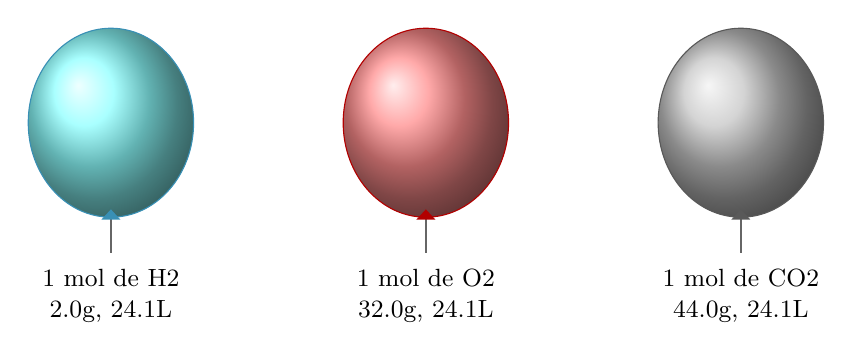
\begin{tikzpicture}[font=\small]
  \foreach \x/\g/\m/\c in {0/{\ce{H2}}/2.0/cyan, 4/{\ce{O2}}/32.0/red,
                           8/{\ce{CO2}}/44.0/gray} {
    \draw[thick, black!60] (\x,-0.25) -- (\x,-1.1);
    \shade[ball color=\c!45, draw=\c!70!black] (\x,0.55) ellipse (1.05 and 1.2);
    \fill[\c!70!black] (\x-0.12,-0.68) -- (\x+0.12,-0.68) -- (\x,-0.55) -- cycle;
    \node[align=center] at (\x,-1.65) {1 mol de \g\\ \qty{\m}{g},
      \qty{24.1}{L}};
  }
\end{tikzpicture}

{\small Trois ballons à \qty{20}{\celsius}, contenant chacun une \omterm{def:g10:the-mole:amount}{mole}
d'un gaz différent. Les volumes sont les mêmes~; les masses, non.}
\end{omfigure}


\begin{example}[Un ballon de dioxyde de carbone]\label{ex:g10:the-mole:balloon}
% ledger: aw:C, aw:O
Un ballon contient \qty{2.4}{L} de dioxyde de carbone à
\qty{20}{\celsius}. Sa \omterm{def:g10:the-mole:amount}{quantité de matière} est
$n = \qty{2.4}{L} / \qty{24.1}{L/mol} = \qty{0.10}{mol}$,
et sa masse $m = \qty{0.10}{mol} \times \qty{44.0}{g/mol} =
\qty{4.4}{g}$. Le même ballon rempli de dihydrogène contiendrait les
mêmes \qty{0.10}{mol}, mais seulement \qty{0.20}{g} de gaz.
\end{example}

\begin{remark}[Gaz lourds et gaz légers]\label{rem:g10:the-mole:heavy}
Comme un litre de n'importe quel gaz contient la même \omterm{def:g10:the-mole:amount}{quantité de
matière}, la masse d'un litre de gaz est proportionnelle à sa \omterm{def:g10:the-mole:molar-mass}{masse
molaire}. L'\omterm{def:g4:air-a-mixture-of-gases:air}{air}, un \omterm{def:g6:pure-substances-and-mixtures:mixture}{mélange} d'environ quatre cinquièmes de diazote
(\qty{28.0}{g/mol}) et d'un cinquième de dioxygène (\qty{32.0}{g/mol}),
se comporte comme un gaz de \omterm{def:g10:the-mole:molar-mass}{masse molaire} voisine de \qty{29}{g/mol}. Un
gaz de \omterm{def:g10:the-mole:molar-mass}{masse molaire} plus grande, comme le dioxyde de carbone
(\qty{44.0}{g/mol}), est plus dense que l'\omterm{def:g4:air-a-mixture-of-gases:air}{air} et s'accumule au fond d'une
cave fermée~; un gaz de \omterm{def:g10:the-mole:molar-mass}{masse molaire} plus petite, comme l'hélium
(\qty{4.0}{g/mol}), s'élève.
\end{remark}

\section{Exercices}

\begin{exercise}[$\star$]\label{exo:g10:the-mole:1}
Calculer les \omterm{def:g10:the-mole:molar-mass}{masses molaires} du dioxygène \ce{O2}, du diazote \ce{N2}, du
méthane \ce{CH4}, de l'ammoniac \ce{NH3} et du dioxyde de carbone
\ce{CO2}.
\end{exercise}

\begin{exercise}[$\star$]\label{exo:g10:the-mole:2}
Quelle \omterm{def:g10:the-mole:amount}{quantité de matière} contiennent \qty{36.0}{g} d'eau~? Et
\qty{4.0}{g} de méthane~?
\end{exercise}

\begin{exercise}[$\star$]\label{exo:g10:the-mole:3}
Quelle est la masse de \qty{0.25}{mol} de chlorure de sodium \ce{NaCl}~?
Et celle de \qty{2.0}{mol} de dioxyde de carbone~?
\end{exercise}

\begin{exercise}[$\star$]\label{exo:g10:the-mole:4}
Combien y a-t-il de \omterm{def:g7:atoms-and-molecules:molecule}{molécules} dans \qty{0.50}{mol} de dioxygène~? Quelle
quantité de fer contient \num{3.0e24} \omterm{def:g7:atoms-and-molecules:atom}{atomes} de fer~?
\end{exercise}

\begin{exercise}[$\star$]\label{exo:g10:the-mole:5}
À \qty{20}{\celsius} et sous la pression atmosphérique normale, quel
volume occupent \qty{0.50}{mol} de diazote~? Quelle quantité de
dioxygène y a-t-il dans \qty{12}{L} de ce gaz~?
\end{exercise}

\begin{exercise}[$\star\star$]\label{exo:g10:the-mole:6}
Une goutte d'eau a un volume de \qty{0.050}{mL}, et \qty{1}{mL} d'eau a
une masse de \qty{1.0}{g}. Combien de \omterm{def:g7:atoms-and-molecules:molecule}{molécules} d'eau la goutte
contient-elle~?
\end{exercise}

\begin{exercise}[$\star\star$]\label{exo:g10:the-mole:7}
Qu'est-ce qui contient le plus d'\omterm{def:g7:atoms-and-molecules:atom}{atomes}, \qty{10}{g} d'aluminium ou
\qty{10}{g} de fer~? Répondre d'abord sans calcul, puis vérifier par le
calcul.
\end{exercise}

\begin{exercise}[$\star\star$]\label{exo:g10:the-mole:8}
À \qty{20}{\celsius}, calculer la masse d'un litre de dioxyde de
carbone et celle d'un litre de diazote. Pourquoi le dioxyde de carbone
s'accumule-t-il au fond d'une cave fermée où fermente du jus de
raisin~?
\end{exercise}

\begin{exercise}[$\star\star$]\label{exo:g10:the-mole:9}
À l'aide de la figure des trois cases $m$, $n$, $N$, donner la masse de
\num{1.0e22} \omterm{def:g7:atoms-and-molecules:molecule}{molécules} de glucose \ce{C6H12O6}. Indiquer les deux
flèches suivies.
\end{exercise}

\begin{exercise}[$\star\star$]\label{exo:g10:the-mole:10}
Un morceau de sucre (saccharose, \ce{C12H22O11}) a une masse de
\qty{5.0}{g}. Calculer la quantité de saccharose qu'il contient, puis
le nombre de \omterm{def:g7:atoms-and-molecules:molecule}{molécules} de saccharose, puis le nombre d'\omterm{def:g7:atoms-and-molecules:atom}{atomes} de
carbone.
\end{exercise}

\begin{exercise}[$\star\star$]\label{exo:g10:the-mole:11}
Qu'est-ce qui contient la plus grande quantité de \omterm{def:g7:atoms-and-molecules:molecule}{molécules}~:
\qty{1.0}{kg} d'eau \ce{H2O} ou \qty{1.0}{kg} d'éthanol \ce{C2H6O}~?
Dans quel rapport~?
\end{exercise}

\begin{exercise}[$\star\star\star$]\label{exo:g10:the-mole:12}
Une bague en or a une masse de \qty{5.0}{g}~; les trois quarts de sa
masse sont de l'or, le reste du cuivre. Combien d'\omterm{def:g7:atoms-and-molecules:atom}{atomes} d'or
contient-elle~? Combien d'\omterm{def:g7:atoms-and-molecules:atom}{atomes} de cuivre~? Quel \omterm{def:g9:periodic-table-first-look:metal}{métal} a le plus
d'\omterm{def:g7:atoms-and-molecules:atom}{atomes} dans la bague~?
\end{exercise}

\begin{exercise}[$\star\star\star$]\label{exo:g10:the-mole:13}
Une salle de classe mesure \qty{8.0}{m} sur \qty{6.0}{m} sur
\qty{3.0}{m}, et l'\omterm{def:g4:air-a-mixture-of-gases:air}{air} qu'elle contient est à \qty{20}{\celsius}.
\begin{enumerate}
  \item Quelle quantité de gaz contient-elle
        ($\qty{1}{m^3} =
        \qty{1000}{L}$)~? Combien de \omterm{def:g7:atoms-and-molecules:molecule}{molécules}~?
  \item En considérant l'\omterm{def:g4:air-a-mixture-of-gases:air}{air} comme formé, sur cent \omterm{def:g7:atoms-and-molecules:molecule}{molécules}, de 78
        \omterm{def:g7:atoms-and-molecules:molecule}{molécules} de diazote, 21 de dioxygène et 1 d'argon
        (\qty{40.0}{g/mol}), calculer la \omterm{def:g10:the-mole:molar-mass}{masse molaire} moyenne de
        l'\omterm{def:g4:air-a-mixture-of-gases:air}{air}.
  \item Quelle est la masse de l'\omterm{def:g4:air-a-mixture-of-gases:air}{air} de la salle~?
\end{enumerate}
\end{exercise}

\begin{exercise}[$\star\star\star$]\label{exo:g10:the-mole:14}
Une sphère de silicium pur a une masse d'exactement \qty{1.000}{kg}.
\begin{enumerate}
  \item Combien d'\omterm{def:g7:atoms-and-molecules:atom}{atomes} de silicium contient-elle~?
  \item En déduire la masse d'un \omterm{def:g7:atoms-and-molecules:atom}{atome} de silicium.
  \item Avant 2019, la \omterm{def:g10:the-mole:avogadro}{constante d'Avogadro} n'était pas fixée mais
        mesurée. Expliquer comment un comptage indépendant des \omterm{def:g7:atoms-and-molecules:atom}{atomes}
        d'une telle sphère, dont la \omterm{def:g10:the-mole:amount}{quantité de matière} est connue par sa
        masse, en donnerait une valeur.
\end{enumerate}
\end{exercise}

\begin{exercise}[$\star\star\star$]\label{exo:g10:the-mole:15}
% ledger: iso:Cl35, iso:Cl37
Le chlore naturel contient \qty{75.8}{\percent} d'\omterm{def:g7:atoms-and-molecules:atom}{atomes} de chlore~35,
de \omterm{def:g10:the-mole:molar-mass}{masse molaire} très proche de \qty{35.0}{g/mol}, et
\qty{24.2}{\percent} d'\omterm{def:g7:atoms-and-molecules:atom}{atomes} de chlore~37, de \omterm{def:g10:the-mole:molar-mass}{masse molaire} très proche
de \qty{37.0}{g/mol}. Calculer la \omterm{def:g10:the-mole:molar-mass}{masse molaire atomique} du chlore
naturel, et la comparer à la valeur du tableau.
\end{exercise}

\section{Problème~: le verre d'eau de Kelvin}

\begin{problem}[{Problème du week-end --- verser un verre d'eau dans la
mer, attendre qu'il se mélange à tous les océans, puis remplir de
nouveau le verre~: combien des premières molécules reviennent~?}]
\label{pb:g10:the-mole:1}
% ledger: ocean:volume, rho:water, const:NA, aw:H, aw:O
Une célèbre expérience de pensée, souvent attribuée au physicien Lord
Kelvin, se déroule ainsi. On marque chaque \omterm{def:g7:atoms-and-molecules:molecule}{molécule} d'un verre d'eau, on
verse le verre dans la mer, et on attend que les \omterm{def:g7:atoms-and-molecules:molecule}{molécules} marquées se
soient réparties uniformément dans tous les océans du monde. On replonge
alors le verre dans la mer, n'importe où. Rapportera-t-il des \omterm{def:g7:atoms-and-molecules:molecule}{molécules}
marquées~? Le verre contient \qty{250}{mL}, et \qty{1}{mL} d'eau a une
masse de \qty{1.0}{g}. Les océans contiennent environ
\qty{1.335e9}{km^3} d'eau. On assimilera l'eau de mer à de l'eau pure
pour le décompte.

\medskip
\noindent\textbf{Partie I --- L'eau d'un verre.}
\begin{enumerate}
  \item Calculer la \omterm{def:g10:the-mole:molar-mass}{masse molaire} de l'eau.
  \item Quelle est la masse de l'eau du verre~?
  \item Calculer la quantité de \omterm{def:g7:atoms-and-molecules:molecule}{molécules} d'eau du verre.
  \item Quelle quantité d'\omterm{def:g7:atoms-and-molecules:atom}{atomes} d'hydrogène le verre contient-il~? Et
        d'\omterm{def:g7:atoms-and-molecules:atom}{atomes} d'oxygène~?
\end{enumerate}

\medskip
\noindent\textbf{Partie II --- Les \omterm{def:g7:atoms-and-molecules:molecule}{molécules} du verre.}
\begin{enumerate}[resume]
  \item Combien de \omterm{def:g7:atoms-and-molecules:molecule}{molécules} d'eau le verre contient-il~?
  \item Calculer la masse d'une \omterm{def:g7:atoms-and-molecules:molecule}{molécule} d'eau, en grammes.
  \item Vérifier les réponses aux questions 5 et 6 en les multipliant~:
        que doit valoir le produit~?
  \item En comptant une \omterm{def:g7:atoms-and-molecules:molecule}{molécule} par seconde, jour et nuit, combien
        d'années faudrait-il pour compter les \omterm{def:g7:atoms-and-molecules:molecule}{molécules} du verre~? (Une
        année dure environ \qty{3.16e7}{s}.)
\end{enumerate}

\medskip
\noindent\textbf{Partie III --- L'océan.}
\begin{enumerate}[resume]
  \item Convertir le volume des océans en mètres cubes
        ($\qty{1}{km^3} = \qty{e9}{m^3}$), puis en litres.
  \item Une fois les \omterm{def:g7:atoms-and-molecules:molecule}{molécules} marquées réparties uniformément, combien
        y en a-t-il dans chaque litre d'océan~?
  \item Combien de \omterm{def:g7:atoms-and-molecules:molecule}{molécules} marquées le second verre rapporte-t-il~?
  \item Seconde méthode. Calculer la quantité d'eau des océans, en
        prenant \qty{1.0}{kg} pour la masse d'un litre.
  \item Quelle fraction de toutes les \omterm{def:g7:atoms-and-molecules:molecule}{molécules} d'eau de l'océan est
        marquée~?
  \item Multiplier cette fraction par le nombre de \omterm{def:g7:atoms-and-molecules:molecule}{molécules} du second
        verre, et comparer avec la réponse à la question 11.
\end{enumerate}

\medskip
\noindent\textbf{Partie IV --- Ce que cela signifie.}
\begin{enumerate}[resume]
  \item Combien de verres de \qty{250}{mL} pourrait-on remplir avec
        l'eau des océans~?
  \item Comparer ce nombre au nombre de \omterm{def:g7:atoms-and-molecules:molecule}{molécules} d'un verre. Expliquer
        en une phrase pourquoi le second verre rapporte autant de
        \omterm{def:g7:atoms-and-molecules:molecule}{molécules} marquées.
  \item Quel volume d'eau de mer faut-il prélever, en moyenne, pour
        rapporter une seule \omterm{def:g7:atoms-and-molecules:molecule}{molécule} marquée~? Comparer avec une goutte
        de \qty{0.05}{mL}.
  \item La réponse à la question 11 comporte beaucoup de chiffres.
        Pourquoi ne faut-il la donner qu'en ordre de grandeur~? Donner
        deux raisons.
  \item Donner la réponse finale~: environ combien de \omterm{def:g7:atoms-and-molecules:molecule}{molécules} du
        premier verre reviennent dans le second~?
\end{enumerate}
\end{problem}
